\documentclass[14pt]{beamer}
\usepackage{./Estilos/BeamerUVM}
\usepackage{./Estilos/ColoresLatex}
\input{Preambulos/preambulo_Beamer_Cambridge_wolverine}
% \usefonttheme{serif}
\usepackage[clock]{ifsym}
\DeclareSIUnit\erg{erg}
\DeclareSIUnit[number-unit-product = {\,}]\cal{cal}

\sisetup{per-mode=symbol}
\resetcounteronoverlays{saveenumi}

\title{\Large{Electricidad y Magnetismo} \\ \normalsize{Física 2}}
\date{24 de julio de 2023}

\begin{document}
\maketitle

\section*{Contenido}
\frame[allowframebreaks]{\frametitle{Contenido} \tableofcontents[currentsection, hideallsubsections]}

\section{Electricidad}
\frame[allowframebreaks]{\tableofcontents[currentsection, hideothersubsections]}
\subsection{Introducción}

\begin{frame}
\frametitle{Preguntas disparadoras}
¿Te has imaginado vivir en un mundo sin energía eléctrica?
\\
\bigskip
\pause
Esto implicaría no usar aparatos electrónicos como radio, televisión, grabadora y otros más.
\end{frame}
\begin{frame}
\frametitle{Nooooo!}
\begin{figure}
    \centering
    \includegraphics[scale=0.1]{Imagenes/emoji_sorpresa.jpg}
\end{figure}
\end{frame}
\begin{frame}
\frametitle{Aprovechamiento de la electricidad}
Por lo tanto, \pause contar con un tipo de fuente de energía, empleando una propiedad física, \pause nos facilita y mejora nuestra calidad de vida, porque sin ella, no contaríamos con iluminación
y calor.
\end{frame}
\begin{frame}
\frametitle{Aprovechamiento de la electricidad}
Esto significa que con esta fuente de energía se ponen en marcha diferentes tipos de máquinas, artefactos y sistemas de transporte, por mencionar algunos.
\end{frame}
\begin{frame}
\frametitle{¿Qué es la electricidad?}
La palabra electricidad se deriva de la raíz griega elektron, que significa ámbar.
\end{frame}
\begin{frame}
\frametitle{¿Qué es la electricidad?}
La electricidad se define como un fenómeno físico que se origina del \textocolor{flame}{movimiento de partículas subatómicas por medio de cargas eléctricas} a través de la atracción y repulsión de las mismas.
\end{frame}
\begin{frame}
\frametitle{¿Qué es la electricidad?}
la Electricidad es una rama de la Física que estudia todos los fenómenos relacionados con las cargas eléctricas en reposo o movimiento.
\end{frame}
\begin{frame}
\frametitle{Electrostática}
Rama de la electricidad que se encarga de estudiar las \textocolor{folly}{cargas eléctricas en reposo}.
\end{frame}
\begin{frame}
\frametitle{Electrodinámica}
Es la rama de la electricidad que se encarga de estudiar las \textocolor{halayaube}{cargas eléctricas en movimiento}.
\end{frame}
\begin{frame}
\frametitle{Propiedad fundamental}
La \textocolor{hanpurple}{carga eléctrica} es una propiedad fundamental de la materia y base de todos los fenómenos de interacción eléctrica.
\\
\bigskip
\pause
Se representa con la letra $q$.
\end{frame}
\begin{frame}
\frametitle{Tipos de carga eléctrica}
Las cargas eléctricas son de dos tipos:
\pause
\begin{figure}
    \centering
    \begin{tikzpicture}
        \node at (0, 0) {Tipos de carga};
        \draw node at (4.75, 1) {Carga positiva};
        \draw [-stealth] (2, 0) -- (3, 1);
        \draw [fill, color=ao, text=white] (7.5, 1) circle (10pt) node {$+$};

        \draw node at (4.75, -1) {Carga negativa};
        \draw [-stealth] (2, 0) -- (3, -1);
        \draw [fill, color=red, text=white] (7.5, -1) circle (10pt) node {$-$};
        
    \end{tikzpicture}
\end{figure}
\end{frame}
\begin{frame}
\frametitle{La carga eléctrica}
Se denomina \textocolor{ballblue}{carga eléctrica elemental} y se denota como:
\pause
\begin{itemize}
\item Carga positiva $+e$, $e^{+}$
\item Carga negativa $-e$, $e^{-}$
\end{itemize}
\end{frame}
\begin{frame}
\frametitle{El valor de $e$}
El valor de la carga eléctrica $e$ es:
\pause
\begin{align*}
e = \SI{1.6d-19}{\coulomb}
\end{align*}
\pause
Entonces:
\begin{itemize}
\item Carga positiva $+e, \, e^{+} = + \SI{1.6d-19}{\coulomb}$
\item Carga negativa $-e, \, e^{-} = -\SI{1.6d-19}{\coulomb}$
\end{itemize}    
\end{frame}
\begin{frame}
\frametitle{Interacción entre cargas eléctricas}
La relación entre cargas eléctricas con signo, se presenta a continuación:
\end{frame}
\begin{frame}
\frametitle{Ley de atracción}
\textocolor{airforceblue}{Cargas con signo contrario se atraen}.
\begin{figure}
    \centering
    \begin{tikzpicture}
        \draw [fill, color=ao, text=white] (0, 0) circle (10pt) node {$+$};
        \draw[-{Triangle[width=18pt,length=8pt]}, line width=10pt](1, 0) -- (2, 0);
        \draw[-{Triangle[width=18pt,length=8pt]}, line width=10pt](4, 0) -- (3, 0);
        \draw [fill, color=red, text=white] (5, 0) circle (10pt) node {$-$};
    \end{tikzpicture}
\end{figure}
\end{frame}
\begin{frame}
\frametitle{Ley de repulsión}
\textocolor{ao(english)}{Cargas con signo igual se repelen}.
\begin{figure}
    \centering
    \begin{tikzpicture}
        \draw [fill, color=ao, text=white] (0, 0) circle (10pt) node {$+$};
        \draw[-{Triangle[width=18pt,length=8pt]}, line width=10pt](-0.5, 0) -- (-1.5, 0);
        \draw[-{Triangle[width=18pt,length=8pt]}, line width=10pt](3, 0) -- (4, 0);
        \draw [fill, color=ao, text=white] (2.5, 0) circle (10pt) node {$+$};

        \draw [fill, color=red, text=white] (0, -1.5) circle (10pt) node {$-$};
        \draw[-{Triangle[width=18pt,length=8pt]}, line width=10pt](-0.5, -1.5) -- (-1.5, -1.5);
        \draw[-{Triangle[width=18pt,length=8pt]}, line width=10pt](3, -1.5) -- (4, -1.5);
        \draw [fill, color=red, text=white] (2.5, -1.5) circle (10pt) node {$-$};
        
    \end{tikzpicture}
\end{figure}
\end{frame}
\begin{frame}
\frametitle{Pregunta interesante}
¿Por qué el núcleo de un átomo no se desintegra si dentro se tienen los protones? Es decir, partículas con carga positiva. 
\end{frame}
\begin{frame}
\frametitle{La carga en la naturaleza}
La experiencia nos dice que los materiales tienen un \textocolor{blue(pigment)}{equilibrio en su carga eléctrica}, \pause es decir, son \textocolor{byzantium}{neutros}.
\end{frame}
\begin{frame}
\frametitle{¿De dónde viene la carga eléctrica?}
La carga eléctrica de un cuerpo aparece cuando éste \textocolor{burgundy}{pierde} o \textocolor{carmine}{gana} electrones, \pause y se dice que cualquier carga eléctrica de magnitud $q$ es un múltiplo entero de la carga elemental $e$, es decir:
\pause
\begin{align*}
q = n \, e \hspace{1cm} \left[ \unit{\coulomb} \,\, (\text{Coulomb}) \right]
\end{align*}
\end{frame}
\begin{frame}
\frametitle{Ejercicio con carga eléctrica}
Un día lluvioso hay una tormenta eléctrica, cae un rayo en un árbol, el cual transfiere una carga de \SI{200}{\coulomb} al árbol.
\\
\bigskip
\pause
¿Cuántos electrones se transfieren al árbol?
\end{frame}
\begin{frame}
\frametitle{Resolviendo el ejercicio}
\textocolor{red}{Datos:}
\begin{align*}
q &= - \SI{200}{\coulomb} \\[0.5em]
e &= - \SI{1.6d-19}{\coulomb}
\end{align*}
\end{frame}
\begin{frame}
\frametitle{Resolviendo el Ejercicio}
\textocolor{red}{Expresión:} \pause \quad $q = n \, e$ \pause \quad $n =\dfrac{q}{e}$
\pause
\\
\textocolor{red}{Sustitución:}
\begin{eqnarray*}
\begin{aligned}
n = \dfrac{- \SI{200}{\coulomb}}{- \SI{1.6d-19}{\coulomb}} = \pause \num{1.25d21} \, \text{electrones}
\end{aligned}
\end{eqnarray*}
\end{frame}
\begin{frame}
\frametitle{Una ley importante}
\textocolor{ceruleanblue}{Conservación de la carga eléctrica}.
\\
\bigskip
La carga eléctrica no se crea ni se destruye, solo se transforma de un cuerpo o material a otro.
\end{frame}

\section{Tipos de materiales}
\frame[allowframebreaks]{\tableofcontents[currentsection, hideothersubsections]}
\subsection{Conductor}

\begin{frame}
\frametitle{El material conductor}
Un medio o material que \textocolor{burgundy}{permite el movimiento} de las cargas eléctricas (electrones)
en respuesta a una fuerza eléctrica, se denomina \textocolor{cobalt}{conductor}.
\end{frame}
\begin{frame}
\frametitle{El material conductor}    
Los materiales conductores son los que se pueden electrizar en toda su superficie, debido a que los electrones se mueven libremente.
\\
\bigskip
\pause
Los metales por lo general son buenos conductores de la electricidad.
\end{frame}
\begin{frame}
\frametitle{Materiales conductores}
\begin{figure}
    \centering
    \includegraphics[scale=0.8]{Imagenes/Materiales_Conductores_01.jpg}
\end{figure}
\end{frame}
\begin{frame}
\frametitle{La corriente eléctrica}
El flujo de las partículas cargadas es lo que se conoce como \textocolor{red}{corriente eléctrica}.
\end{frame}
\begin{frame}
\frametitle{La corriente eléctrica}
Las partículas cargadas en una cierta dirección de un conductor chocan con los átomos, \pause produciendo una pérdida de energía que se manifiesta en forma de calor.
\end{frame}
\begin{frame}
\frametitle{La resistencia eléctrica}
Una medida de \textocolor{blue}{oposición} que presentan las partículas cargadas al moverse libremente en una cierta dirección de un material conductor \pause es lo que se conoce como \textocolor{cerise}{resistencia eléctrica}.
\end{frame}
\begin{frame}
\frametitle{Materiales resistivos}
\begin{figure}
    \centering
    \includegraphics[scale=0.3]{Imagenes/Materiales_Conductores_02.jpg}
\end{figure}
\end{frame}
    
\subsection{Aislante}

\begin{frame}
\frametitle{Los aislantes}
Los materiales que no permiten que las partículas cargadas se muevan hacia otra región del material debido a una fuerza eléctrica, son llamados \textocolor{coolblack}{aislantes} por ejemplo, la madera.
\end{frame}

\subsection{Semiconductores}

\begin{frame}
\frametitle{Los materiales semiconductores}
Existen otros tipos de materiales cuyas propiedades son intermedias entre los conductores y aislantes: \pause  se llaman \textocolor{cornellred}{semiconductores}.
\end{frame}
\begin{frame}
\frametitle{Base de la electrónica}
Los materiales semiconductores con mayor utilidad en la electrónica son el silicio y el germanio.
\end{frame}

\section{Ley de Coulomb}
\frame[allowframebreaks]{\tableofcontents[currentsection, hideothersubsections]}
\subsection{Fuerza entre cargas}

\begin{frame}
\frametitle{La ley de Coulomb}
La ley de Coulomb establece que la fuerza $F$, con que dos cargas eléctricas $q_{1}$ y $q_{2}$ se atraen o repelen \pause es \textocolor{darkgreen}{proporcional} al producto de las mismas \pause e \textocolor{darkmagenta}{inversamente proporcional} al cuadrado de la distancia $r$ que las separa.
\end{frame}
\begin{frame}
\frametitle{Expresión para la ley de Coulomb}
La expresión es la siguiente:
\pause
\begin{align*}
F = k \, \dfrac{q_{1} \, q_{2}}{r^{2}}
\end{align*}
donde:
\pause
\begin{itemize}[<+->]
\item $k$ es una constante de proporcionalidad, tal que:
\begin{align*}
k = \SI[per-mode=fraction]{9d9}{\newton\square\meter\per\square\coulomb}
\end{align*}
para el vacío.
\end{itemize}
\end{frame}
\begin{frame}
\frametitle{Caso donde se cumple}
La ley de Coulomb se cumple cuando las cargas se encuentran \textocolor{darkolivegreen}{en el vacío}, \pause pues si el medio es el aire, aceite, etc., la fuerza electrostática se reduce considerablemente.
\end{frame}
\begin{frame}
\frametitle{Relación entre el vacío y otro medio}
La relación que existe entre la fuerza en el vacío $F$ y la fuerza en otro medio $F_{m}$, \pause se conoce como \textocolor{darkraspberry}{permitividad relativa del medio}, la cual se expresa matemáticamente:
\pause
\begin{align*}
\varepsilon = \dfrac{F}{F_{m}}
\end{align*}
\end{frame}
\begin{frame}
\frametitle{Valores de permitividad}
\begin{table}
\centering
\begin{tabular}{c | c}
Material & $\varepsilon$ \\ \hline
Vacío & $1$ \\ \hline
Aire & $1.006$ \\ \hline
Vidrio & $7$ \\ \hline
Mica & $5$ \\ \hline    
\end{tabular}
\end{table}
\end{frame}
\begin{frame}
\frametitle{Ejercicio}
¿Cuál es la fuerza eléctrica entre las cargas mostrada en la figura?
\begin{figure}
    \centering
    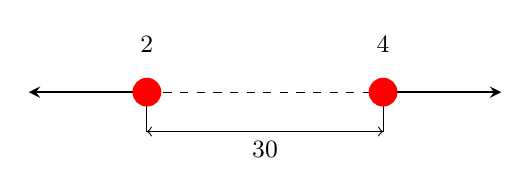
\begin{tikzpicture}
        \draw (0, 0) -- (0, -0.5);
        \draw (3, 0) -- (3, -0.5);

        \draw [dashed] (0, 0) -- (3, 0);

        \draw[-stealth, thick] (0, 0) -- (-1.5, 0);
        \draw [fill, color=red] (0, 0) circle (5pt);
        \draw[-stealth, thick] (3, 0) -- (4.5, 0);
        \draw [fill, color=red] (3, 0) circle (5pt);

        \draw [<->] (0, -0.5) -- (3, -0.5) node [below, midway] {\small{$\SI{30}{\centi\meter}$}};

        \node at (0, 0.6) {\small{$\SI{2}{\micro\coulomb}$}};
        \node at (3, 0.6) {\small{$\SI{4}{\micro\coulomb}$}};

    \end{tikzpicture}
\end{figure}
Considera que se encuentran en el vacío.
\end{frame}
\begin{frame}
\frametitle{Resolviendo el ejercicio}
\textocolor{red}{Datos:}
\pause
\begin{eqnarray*}
\begin{aligned}
q_{1} &= \SI{2}{\micro\coulomb} = \pause \SI{2d-6}{\coulomb} \\[0.3em] \pause
q_{2} &= \SI{4}{\micro\coulomb} = \pause \SI{4d-6}{\coulomb} \\[0.3em] \pause
r &= \SI{30}{\centi\meter} = \pause \SI{0.3}{\meter} \\[0.3em] \pause
k &= \SI[per-mode=fraction]{9d9}{\newton\square\meter\per\square\coulomb} \\[0.3em]
F &= \, ?
\end{aligned}
\end{eqnarray*}
\end{frame}
\begin{frame}
\frametitle{Resolviendo el ejercicio}
\textocolor{red}{Expresión: } \quad \pause $F = k \, \dfrac{q_{1} \, q_{2}}{r^{2}}$
\\[0.5em] \pause
\textocolor{red}{Sustitución: }
\begin{eqnarray*}
\begin{aligned}
F = \left( \SI[per-mode=fraction]{9d9}{\newton\square\meter\per\square\coulomb} \right) \dfrac{\left( \SI{2d-6}{\coulomb} \right) \left( \SI{4d-6}{\coulomb} \right)}{\left( \SI{0.3}{\meter} \right)^{2}} = \pause \SI{0.8}{\newton}
\end{aligned}
\end{eqnarray*}
\end{frame}
\begin{frame}
\frametitle{Enunciado de otro ejercicio}
Determina a qué distancia se deben poner dos cargas iguales de \SI{7d-3}{\coulomb}, para que la fuerza de repulsión sea de \SI{4.4}{\newton}.
\end{frame}
\begin{frame}
\frametitle{Resolviendo el ejercicio}
\textocolor{red}{Datos:}
\pause
\begin{eqnarray*}
\begin{aligned}
q_{1} &= q_{2} = \SI{7d-3}{\coulomb} \\[0.3em] \pause
F &= \SI{4.4}{\newton} \\[0.3em]
k &= \SI[per-mode=fraction]{9d9}{\newton\square\meter\per\square\coulomb} \\[0.3em]
r &= \, ?
\end{aligned}
\end{eqnarray*}
\end{frame}
\begin{frame}
\frametitle{Resolviendo el ejercicio}
\textocolor{red}{Expresión: }
\pause
\begin{eqnarray*}
\begin{aligned}
F &= k \, \dfrac{q_{1} \, q_{2}}{r^{2}} \\[0.5em] \pause
r &= \sqrt{\dfrac{k \, q_{1} \, q_{2}}{F}} = \pause \sqrt{\dfrac{k \, q^{2}}{F}}
\end{aligned}
\end{eqnarray*}
\end{frame}
\begin{frame}
\frametitle{Resolviendo el ejercicio}
\textocolor{red}{Sustitución: }
\begin{eqnarray*}
\begin{aligned}
r &= \sqrt{\dfrac{ \left( \SI[per-mode=fraction]{9d9}{\newton\square\meter\per\square\coulomb} \right) \, \left( \SI{7d-3}{\coulomb} \right)^{2}}{\SI{4.4}{\coulomb}}} = \\[0.5em] \pause
r &= \SI{316.58}{\meter}
\end{aligned}
\end{eqnarray*}
\end{frame}    

\section{Campo eléctrico}
\frame[allowframebreaks]{\tableofcontents[currentsection, hideothersubsections]}
\subsection{Preliminar}

\begin{frame}
\frametitle{De la ley de atracción y repulsión}
Sabemos que las cargas de signos iguales se repelen y de signos diferentes se atraen, esto quiere decir que las cargas influyen sobre la región que está a su alrededor, la cual se conoce como \textocolor{darkspringgreen}{campo eléctrico}.
\end{frame}
\begin{frame}
\frametitle{¿Qué es el campo eléctrico?}
El campo eléctrico es la \textocolor{deepcerise}{zona del espacio donde cargas eléctricas ejercen su influencia}, \pause es decir, que cada carga eléctrica con su presencia modifica las propiedades del espacio que la rodea.
\end{frame}
\begin{frame}
\frametitle{¿Qué es el campo eléctrico?}    
El campo eléctrico es invisible, pero su fuerza ejerce acciones sobre los objetos cargados, lo que permite detectar su presencia y medir su intensidad.
\end{frame}
\begin{frame}
\frametitle{Definición de campo eléctrico}
El campo eléctrico es la región del espacio que rodea al cuerpo cargado eléctricamente y en el que otra carga sentirá una fuerza eléctrica.
\end{frame}
\begin{frame}
\frametitle{Líneas de campo eléctrico}
Las líneas de campo eléctrico son líneas imaginarias trazadas de tal manera que su dirección en cualquier punto es la misma que la dirección del campo eléctrico en ese punto.
\end{frame}
\begin{frame}
\frametitle{Líneas de campo eléctrico}
\begin{figure}
    \centering
    \includegraphics[scale=0.15]{Imagenes/Campo_Electrico_01.png}
\end{figure}
\end{frame}
\begin{frame}
\frametitle{Líneas de campo eléctrico}
\begin{figure}
    \centering
    \includegraphics[scale=0.15]{Imagenes/Campo_Electrico_02.png}
\end{figure}
\end{frame}
\begin{frame}
\frametitle{Líneas de campo eléctrico}
\begin{figure}
    \centering
    \includegraphics[scale=0.1]{Imagenes/Campo_Electrico_03.png}
\end{figure}
\end{frame}

\subsection{Intensidad del campo eléctrico}

\begin{frame}
\frametitle{La intensidad del campo}
La \textocolor{denim}{intensidad del campo eléctrico} $E$ en un punto \pause se suele definir en términos de la
fuerza $F$ que experimenta una carga positiva pequeña $+q$ cuando ésta colocada precisamente en ese punto.
\end{frame}
\begin{frame}
\frametitle{La intensidad del campo}
La magnitud del campo eléctrico ésta dada por:
\pause
\begin{align*}
E = \dfrac{F}{q}
\end{align*}
En el sistema internacional las unidades de la intensidad del campo eléctrico son el newton por coulomb (\unit{\newton\per\coulomb}).
\end{frame}
\begin{frame}
\frametitle{El campo y la ley de Coulomb}
La intensidad del campo eléctrico producida por una carga de prueba puede obtenerse a partir de la ley de Coulomb.
\end{frame}
\begin{frame}
\frametitle{El campo y la ley de Coulomb}
Como la magnitud de la fuerza eléctrica sobre una carga de prueba es:
\pause
\begin{align*}
F &= k \, \dfrac{q_{1} \, q_{2}}{r^{2}}
\end{align*}
\end{frame}
\begin{frame}
\frametitle{Expresión para el campo eléctrico}
Si sustituimos esta expresión de la intensidad y consideramos que $q = q_{0}$:
\pause
\begin{align*}
E = \dfrac{k \, q}{r^{2}}
\end{align*}
\end{frame}
\begin{frame}
\frametitle{Dirección de la intensidad}
La dirección de la intensidad del campo eléctrico $E$ en un punto en el espacio es la misma que la dirección en la que la carga positiva se moverá si se colocara en ese punto.
\end{frame}
\begin{frame}
\frametitle{Dirección de la intensidad}
Alrededor de un cuerpo cargado existe un campo eléctrico, haya o no una segunda carga localizada en el campo.
\end{frame}
\begin{frame}
\frametitle{Fuerza e intensidad de campo eléctrico}
Si una carga se coloca en el campo, experimenta una fuerza $F$ dada por:
\pause
\begin{align*}
F = q \, E
\end{align*}
\end{frame}
\begin{frame}
\frametitle{Enunciado del ejercicio}
Una carga de prueba de \SI{10}{\micro\coulomb} se coloca en un punto del campo eléctrico y la fuerza que experimenta es de \SI{25}{\newton}.
\\
\bigskip
\pause
¿Cuál es la magnitud de la intensidad eléctrica en el punto donde está colocada la carga de prueba?
\end{frame}
\begin{frame}
\frametitle{Resolviendo el ejercicio}
\textocolor{red}{Datos:}
\begin{align*}
q &= \SI{10}{\micro\coulomb} \\[0.5em]
F &= \SI{25}{\newton}
\end{align*}
\end{frame}
\begin{frame}
\frametitle{Resolviendo el ejercicio}
\textocolor{red}{Expresión:} \pause $F = q \, E \hspace{1cm} \Rightarrow \hspace{1cm} E = \dfrac{F}{q}$ \\[0.5em] \pause
\textocolor{red}{Sustitución:} 
\begin{eqnarray*}
\begin{aligned}
E &= \dfrac{\SI{25}{\newton}}{\SI{10d-6}{\coulomb}} = \\[0.5em] \pause 
E &= \SI[per-mode=fraction]{2.5d6}{\newton\per\coulomb}
\end{aligned}
\end{eqnarray*}
\end{frame}
\begin{frame}
\frametitle{Enunciado de otro ejercicio}
Determina el valor de la intensidad del campo eléctrico de una carga de \SI{2}{\micro\coulomb} que se encuentra a una distancia de \SI{40}{\centi\meter} de ésta.
\end{frame}
\begin{frame}
\frametitle{Resolviendo el ejercicio}
\textocolor{red}{Datos:}
\begin{align*}
q &= \SI{2}{\micro\coulomb} \\[0.5em]
k &= \SI[per-mode=fraction]{9d9}{\newton\square\meter\per\square\coulomb} \\[0.5em]
r &= \SI{0.4}{\meter} \\[0.5em]
E &= \, ?
\end{align*}
\end{frame}
\begin{frame}
\frametitle{Resolviendo el ejercicio}
\textocolor{red}{Expresión:} \pause \quad $E = \dfrac{k \, q}{r^{2}}$ \\[0.5em] \pause
\textocolor{red}{Sustitución:} 
\begin{eqnarray*}
\begin{aligned}
E &= \dfrac{\left(\SI[per-mode=fraction]{9d9}{\newton\square\meter\per\square\coulomb}\right)\left(\SI{2d-6}{\coulomb}\right)}{\left(\SI{0.4}{\meter}\right)^{2}} = \\[0.5em] \pause 
E &= \SI[per-mode=fraction]{1.125d5}{\newton\per\coulomb}
\end{aligned}
\end{eqnarray*}
\end{frame}

\section{Electrodinámica}
\frame[allowframebreaks]{\tableofcontents[currentsection, hideothersubsections]}
\subsection{Conceptos}

\begin{frame}
\frametitle{Entendiendo la Electrodinámica}
Ahora estudiaremos los fenómenos relacionados con las \textocolor{red}{cargas en movimiento}, \pause es decir, la \textocolor{ao}{electrodinámica}, \pause la cual se encuentra relacionada con la corriente eléctrica, el potencial eléctrico y la resistencia.
\end{frame}

\subsection{El potencial eléctrico}

\begin{frame}
\frametitle{Definición de potencial eléctrico}
Toda carga eléctrica, positiva o negativa, tiene una \textocolor{blue-violet}{energía potencial eléctrica} debido a su capacidad para realizar trabajo sobre otras cargas. 
\end{frame}
\begin{frame}
\frametitle{Definición de potencial eléctrico}
Cuando una carga es \textocolor{ao}{positiva} se dice que tiene un \textocolor{ao}{potencial positivo}, \pause y si es \textocolor{red}{negativa} tiene un \textocolor{red}{potencial negativo}.
\end{frame}
\begin{frame}
\frametitle{Los potenciales positivo y negativo}
Un potencial es \textocolor{ao}{positivo} si al conectar un cuerpo a tierra, por medio de un conductor eléctrico, \textocolor{ao}{los electrones fluyen desde el suelo al cuerpo}.
\end{frame}
\begin{frame}
\frametitle{Los potenciales positivo y negativo}
El potencial será \textocolor{red}{negativo} si al conectarlo a tierra \textocolor{red}{los electrones fluyen del cuerpo al suelo}.
\\
\bigskip
\pause
En estas definiciones se considera que el potencial eléctrico de la Tierra es cero.
\end{frame}
\begin{frame}
\frametitle{Definición de potencial}
El \textocolor{burgundy}{potencial eléctrico} $V$ en cualquier punto de un campo eléctrico es igual al trabajo $W$ que se necesita realizar para transportar a la unidad de carga positiva $q$ desde el potencial cero hasta el punto considerado.
\end{frame}
\begin{frame}
\frametitle{Expresión para el potencial eléctrico}
La siguiente expresión define el potencial eléctrico:
\pause
\begin{eqnarray*}
\begin{aligned}
V = \dfrac{W}{q} \hspace{0.5cm} \rightarrow \hspace{0.5cm} \left[ \dfrac{\unit{\joule}}{q} \right] \pause \hspace{0.5cm} \rightarrow \hspace{0.5cm} \left[ V \quad \text{volts} \right]
\end{aligned}
\end{eqnarray*}
\end{frame}

\subsection{Diferencia de potencial}

\begin{frame}
\frametitle{La diferencia de potencial}
En términos prácticos, \textocolor{carnelian}{no es tan importante} conocer el potencial eléctrico existente en determinado punto de un campo, \pause sino \textocolor{ceruleanblue}{cuál es la diferencia del potencial eléctrico} entre dos puntos \pause y con ello determinar la cantidad de trabajo necesario para mover cargas eléctricas de un punto a otro.
\end{frame}
\begin{frame}
\frametitle{Definición de diferencia de potencial}
La \textocolor{cobalt}{diferencia de potencial} entre dos puntos cualesquiera $A$ y $B$ \pause es igual al trabajo por unidad de carga positiva que realizan fuerzas eléctricas al mover una carga de prueba desde el punto $A$ al $B$.
\end{frame}
\begin{frame}
\frametitle{Expresión para la diferencia de potencial}
La expresión para el cálculo de la diferencia de potencial es:
\pause
\begin{align*}
V_{AB} = \dfrac{W_{AB}}{q}
\end{align*}
\end{frame}
\begin{frame}
\frametitle{Expresión para la diferencia de potencial}
% \begin{align*}
% V_{AB} = \dfrac{W_{AB}}{q}
% \end{align*}        
Donde:
\setbeamercolor{item projected}{bg=citrine,fg=black}
\setbeamertemplate{enumerate items}{%
\usebeamercolor[bg]{item projected}%
\raisebox{1.5pt}{\colorbox{bg}{\color{fg}\footnotesize\insertenumlabel}}%
}
\begin{enumerate}[<+->]
\item $V_{AB}$ es la diferencia de potencial entre $A$ y $B$, expresada en volts.
\item $W_{AB}$ es el trabajo sobre una carga de prueba $q$ que se desplaza de $A$ a $B$.
\item $q$ es la carga de prueba que se desplaza de $A$ a $B$.
\end{enumerate}
\end{frame}
\begin{frame}
\frametitle{Nombres para la diferencia de potencial}
La diferencia de potencial también recibe los nombres de \textocolor{cadmiumgreen}{voltaje} y de \textocolor{darkgreen}{tensión}.
\\
\bigskip
\pause
Al igual que el potencial eléctrico, la diferencia de potencial es una magnitud escalar.
\end{frame}
\begin{frame}
\frametitle{La diferencia de potencial}
La diferencia de potencial entre dos puntos se puede determinar si se conoce el potencial de cada uno y se obtiene su diferencia.
\end{frame}
\begin{frame}
\frametitle{La diferencia de potencial}    
Veamos: si el potencial en un punto $A$ es de \SI{110}{\volt} \pause y en un punto $B$ es de \SI{60}{\volt}, \pause la diferencia de potencial de $A$ a $B$ es:
\pause
\begin{eqnarray*}
\begin{aligned}
V_{AB} = V_{A} - V_{B} = \pause \SI{110}{\volt} - \SI{60}{\volt} = \pause \SI{50}{\volt}
\end{aligned}
\end{eqnarray*}
\end{frame}

\subsection{La corriente eléctrica}

\begin{frame}
\frametitle{La corriente eléctrica}
Es el \textocolor{bole}{flujo de electrones} que circulan a través un material conductor.
\\
\bigskip
\pause
Se define también como el transporte de carga eléctrica de un punto a otro.
\end{frame}

\subsection{Tipos de corriente}

\begin{frame}
\frametitle{Tipos de corriente}
Dependiendo de cómo sea generada, la corriente eléctrica puede ser de dos tipos:
\pause
\setbeamercolor{item projected}{bg=britishracinggreen,fg=white}
\setbeamertemplate{enumerate items}{%
\usebeamercolor[bg]{item projected}%
\raisebox{1.5pt}{\colorbox{bg}{\color{fg}\footnotesize\insertenumlabel}}%
}
\begin{enumerate}[<+->]
\item La \textocolor{brown(web)}{corriente continua} (o \textocolor{brown(web)}{directa})\pause es aquella en que el flujo de cargas recorre el conductor continuamente, siempre en un mismo sentido.
\seti
\end{enumerate}
\end{frame}
\begin{frame}
\frametitle{La corriente directa}
\textocolor{burntorange}{No varía con el tiempo}.
\\
\bigskip
\pause
Este tipo de corriente es generado por pilas y baterías.
\end{frame}
\begin{frame}
\frametitle{Baterías de corriente directa}
\begin{figure}
    \centering
    \includegraphics[scale=0.6]{Imagenes/Baterias_01.jpg}
\end{figure}
\end{frame}
\begin{frame}
\frametitle{Baterías de corriente directa}
\begin{figure}
    \centering
    \includegraphics[scale=0.4]{Imagenes/Baterias_02.png}
\end{figure}
\end{frame}
\begin{frame}
\frametitle{Gráfica de la corriente directa}
\begin{figure}
    \centering
    \includegraphics[scale=0.7]{Imagenes/Corriente_01.png}
\end{figure}
\end{frame}
\begin{frame}
\frametitle{Pila ya con uso}
¿Cómo será la gráfica de la corriente contra tiempo de una pila/batería que ya ha sido utilizada?
\end{frame}
\begin{frame}
\frametitle{Tipos de corriente}
\setbeamercolor{item projected}{bg=britishracinggreen,fg=white}
\setbeamertemplate{enumerate items}{%
\usebeamercolor[bg]{item projected}%
\raisebox{1.5pt}{\colorbox{bg}{\color{fg}\footnotesize\insertenumlabel}}%
}
\begin{enumerate}[<+->]
\conti
\item La \textocolor{carmine}{corriente alterna} \pause es aquella en que el flujo de cargas se mueve alternadamente dentro del conductor, desplazándose en un sentido y otro.

Este tipo de corriente varía con el tiempo: $I (t)$
\end{enumerate}
\end{frame}
\begin{frame}
\frametitle{Corriente alterna senoidal}
\begin{figure}
    \centering
    \includegraphics[scale=0.7]{Imagenes/Corriente_02.png}
\end{figure}
\end{frame}
\begin{frame}
\frametitle{Corriente alterna triangular}
\begin{figure}
    \centering
    \includegraphics[scale=0.7]{Imagenes/Corriente_04.png}
\end{figure}
\end{frame}
\begin{frame}
\frametitle{Corriente alterna rectangular}
\begin{figure}
    \centering
    \includegraphics[scale=0.7]{Imagenes/Corriente_05.png}
\end{figure}
\end{frame}
\begin{frame}
\frametitle{Corriente alterna}
Este tipo de corriente es producido por generadores eléctricos.
\begin{figure}
    \centering
    \includegraphics[scale=0.7]{Imagenes/Corriente_03.png}
\end{figure}
\end{frame}
\begin{frame}
\frametitle{La intensidad de corriente eléctrica}
Para medir o cuantificar una corriente eléctrica se utiliza el concepto de \textocolor{carmine}{intensidad de corriente eléctrica}.
\end{frame}
\begin{frame}
\frametitle{Definición}
La \textocolor{cerisepink}{intensidad de corriente} (corriente eléctrica) \pause es la carga total que circula a través de la sección transversal de un conductor, por unidad de tiempo.
\end{frame}
\begin{frame}
\frametitle{Expresión}
La expresión matemática que nos permite medir la corriente eléctrica en un conductor:
\pause
\begin{align*}
I = \dfrac{q}{t} \hspace{0.5cm} \rightarrow \hspace{0.5cm} \left[ A \quad (\text{Ampere}) \right]
\end{align*}
\end{frame}
\begin{frame}
\frametitle{Enunciado del ejercicio}
Durante un intervalo de tiempo de \SI{10}{\second}, circula por un conductor una carga de \SI{55}{\coulomb}.
\\
\bigskip
\pause
¿Cuál es la intensidad de la corriente eléctrica?
\end{frame}
\begin{frame}
\frametitle{Resolviendo el ejercicio}
\textocolor{red}{Datos:}
\pause
\begin{align*}
t &= \SI{10}{\second} \\[0.5em]
q &= \SI{55}{\coulomb}
\end{align*}
\end{frame}
\begin{frame}
\frametitle{Resolviendo el ejercicio}
\textocolor{red}{Expresión:} \pause $I = \dfrac{q}{t}$
\pause
\begin{eqnarray*}
\begin{aligned}
I = \dfrac{\SI{55}{\coulomb}}{\SI{10}{\second}} = \pause \SI{5.5}{\ampere}
\end{aligned}
\end{eqnarray*}
\end{frame}

\subsection{La resistencia eléctrica}

\begin{frame}
\frametitle{Definición de resistencia eléctrica}
La \textocolor{coquelicot}{resistencia eléctrica} es la oposición natural que presentan todos los materiales, en mayor o menor medida, al paso de una corriente eléctrica.
\end{frame}
\begin{frame}
\frametitle{Unidades de la resistencia eléctrica}
La resistencia eléctrica se mide en Ohms (\unit{\ohm}), \pause un valor grande en Ohms, nos dice que el material es altamente resistivo.
\end{frame}
\begin{frame}
\frametitle{Definición de resistencia eléctrica}    
Esto se debe a diversos factores como la naturaleza del conductor, \pause por ejemplo, el oro es un buen conductor y opone menos resistencia que el cobre para que circule la corriente.
\end{frame}

\subsection{Ley de Ohm}


\begin{frame}
\frametitle{Definición de la ley de Ohm}
La intensidad de la corriente eléctrica transportada por un conductor es \textocolor{red}{directamente proporcional} a la diferencia de potencial entre sus terminales \pause e \textocolor{cornellred}{inversamente proporcional} a su resistencia eléctrica.
\end{frame}
\begin{frame}
\frametitle{Expresión para la ley de Ohm}
La expresión para la ley de Ohm es:
\pause
\begin{align*}
I = \dfrac{V}{R}
\end{align*}
\end{frame}
\begin{frame}
\frametitle{Ejercicio a resolver}
Determina la intensidad de la corriente eléctrica a través de una corriente eléctrica de \SI{50}{\ohm} al aplicarle un diferencial de potencial de \SI{100}{\volt}.
\end{frame}
\begin{frame}
\frametitle{Ejercicio a resolver}
Calcula la diferencia de potencial aplicada a una resistencia de \SI{20}{\ohm} y por ella fluyen \SI{12}{\ampere}.
\end{frame}

\subsection{La potencia eléctrica}

\begin{frame}
\frametitle{Definición de potencia eléctrica}
La \textocolor{bistre}{potencia eléctrica} mide la cantidad de energía eléctrica que un receptor consume en un tiempo dado.
\end{frame}
\begin{frame}
\frametitle{Expresión para la potencia eléctrica}
La expresión que se utiliza para el cálculo de la potencia es:
\pause
\begin{align*}
P = I \, V \hspace{1cm} \left[ \unit{\watt} \quad \text{Watt} \right]
\end{align*}
\end{frame}

\subsection{Energía eléctrica}

\begin{frame}
\frametitle{Consumo de energía}
Cada mes o dos meses, llega a nuestra casa un recibo \enquote{de la luz}, \pause dependiendo de la cantidad de energía eléctrica que hayamos consumido durante ese período de tiempo.
\end{frame}
\begin{frame}
\frametitle{Consumo de energía}
\begin{figure}
    \centering
    \includegraphics[scale=0.7]{Imagenes/Energia_Electrica_08.jpg}
\end{figure}
\end{frame}
\begin{frame}
\frametitle{Consumo de energía}
Lo que se paga en el recibo, es la suma del consumo por tener conectados y encendidos los electrodomésticos durante cierto tiempo.
\end{frame}
\begin{frame}
\frametitle{Calculando la energía eléctrica}
La energía eléctrica se expresa matemáticamente:
\pause
\begin{align*}
E = P \, t \hspace{1cm} \left[ \unit{\joule} \quad \text{Joule} \right]
\end{align*}
\end{frame}
\begin{frame}
\frametitle{Unidad más utilizada}
Aunque un joule es la unidad en que se mide la energía en el Sistema Internacional (SI), \pause en la práctica, para referirnos al consumo de energía en nuestro hogar o en el comercio, se utiliza la unidad llamada \textocolor{red}{kilowatt-hora} (\SI{1}{\kilo\watt\hour}).
\end{frame}
\end{document}